{
\begin{frame}
    \begin{block}{}
        \begin{center}
            Let's prepare for launch
        \end{center}
    \end{block}
\end{frame}
\usebackgroundtemplate{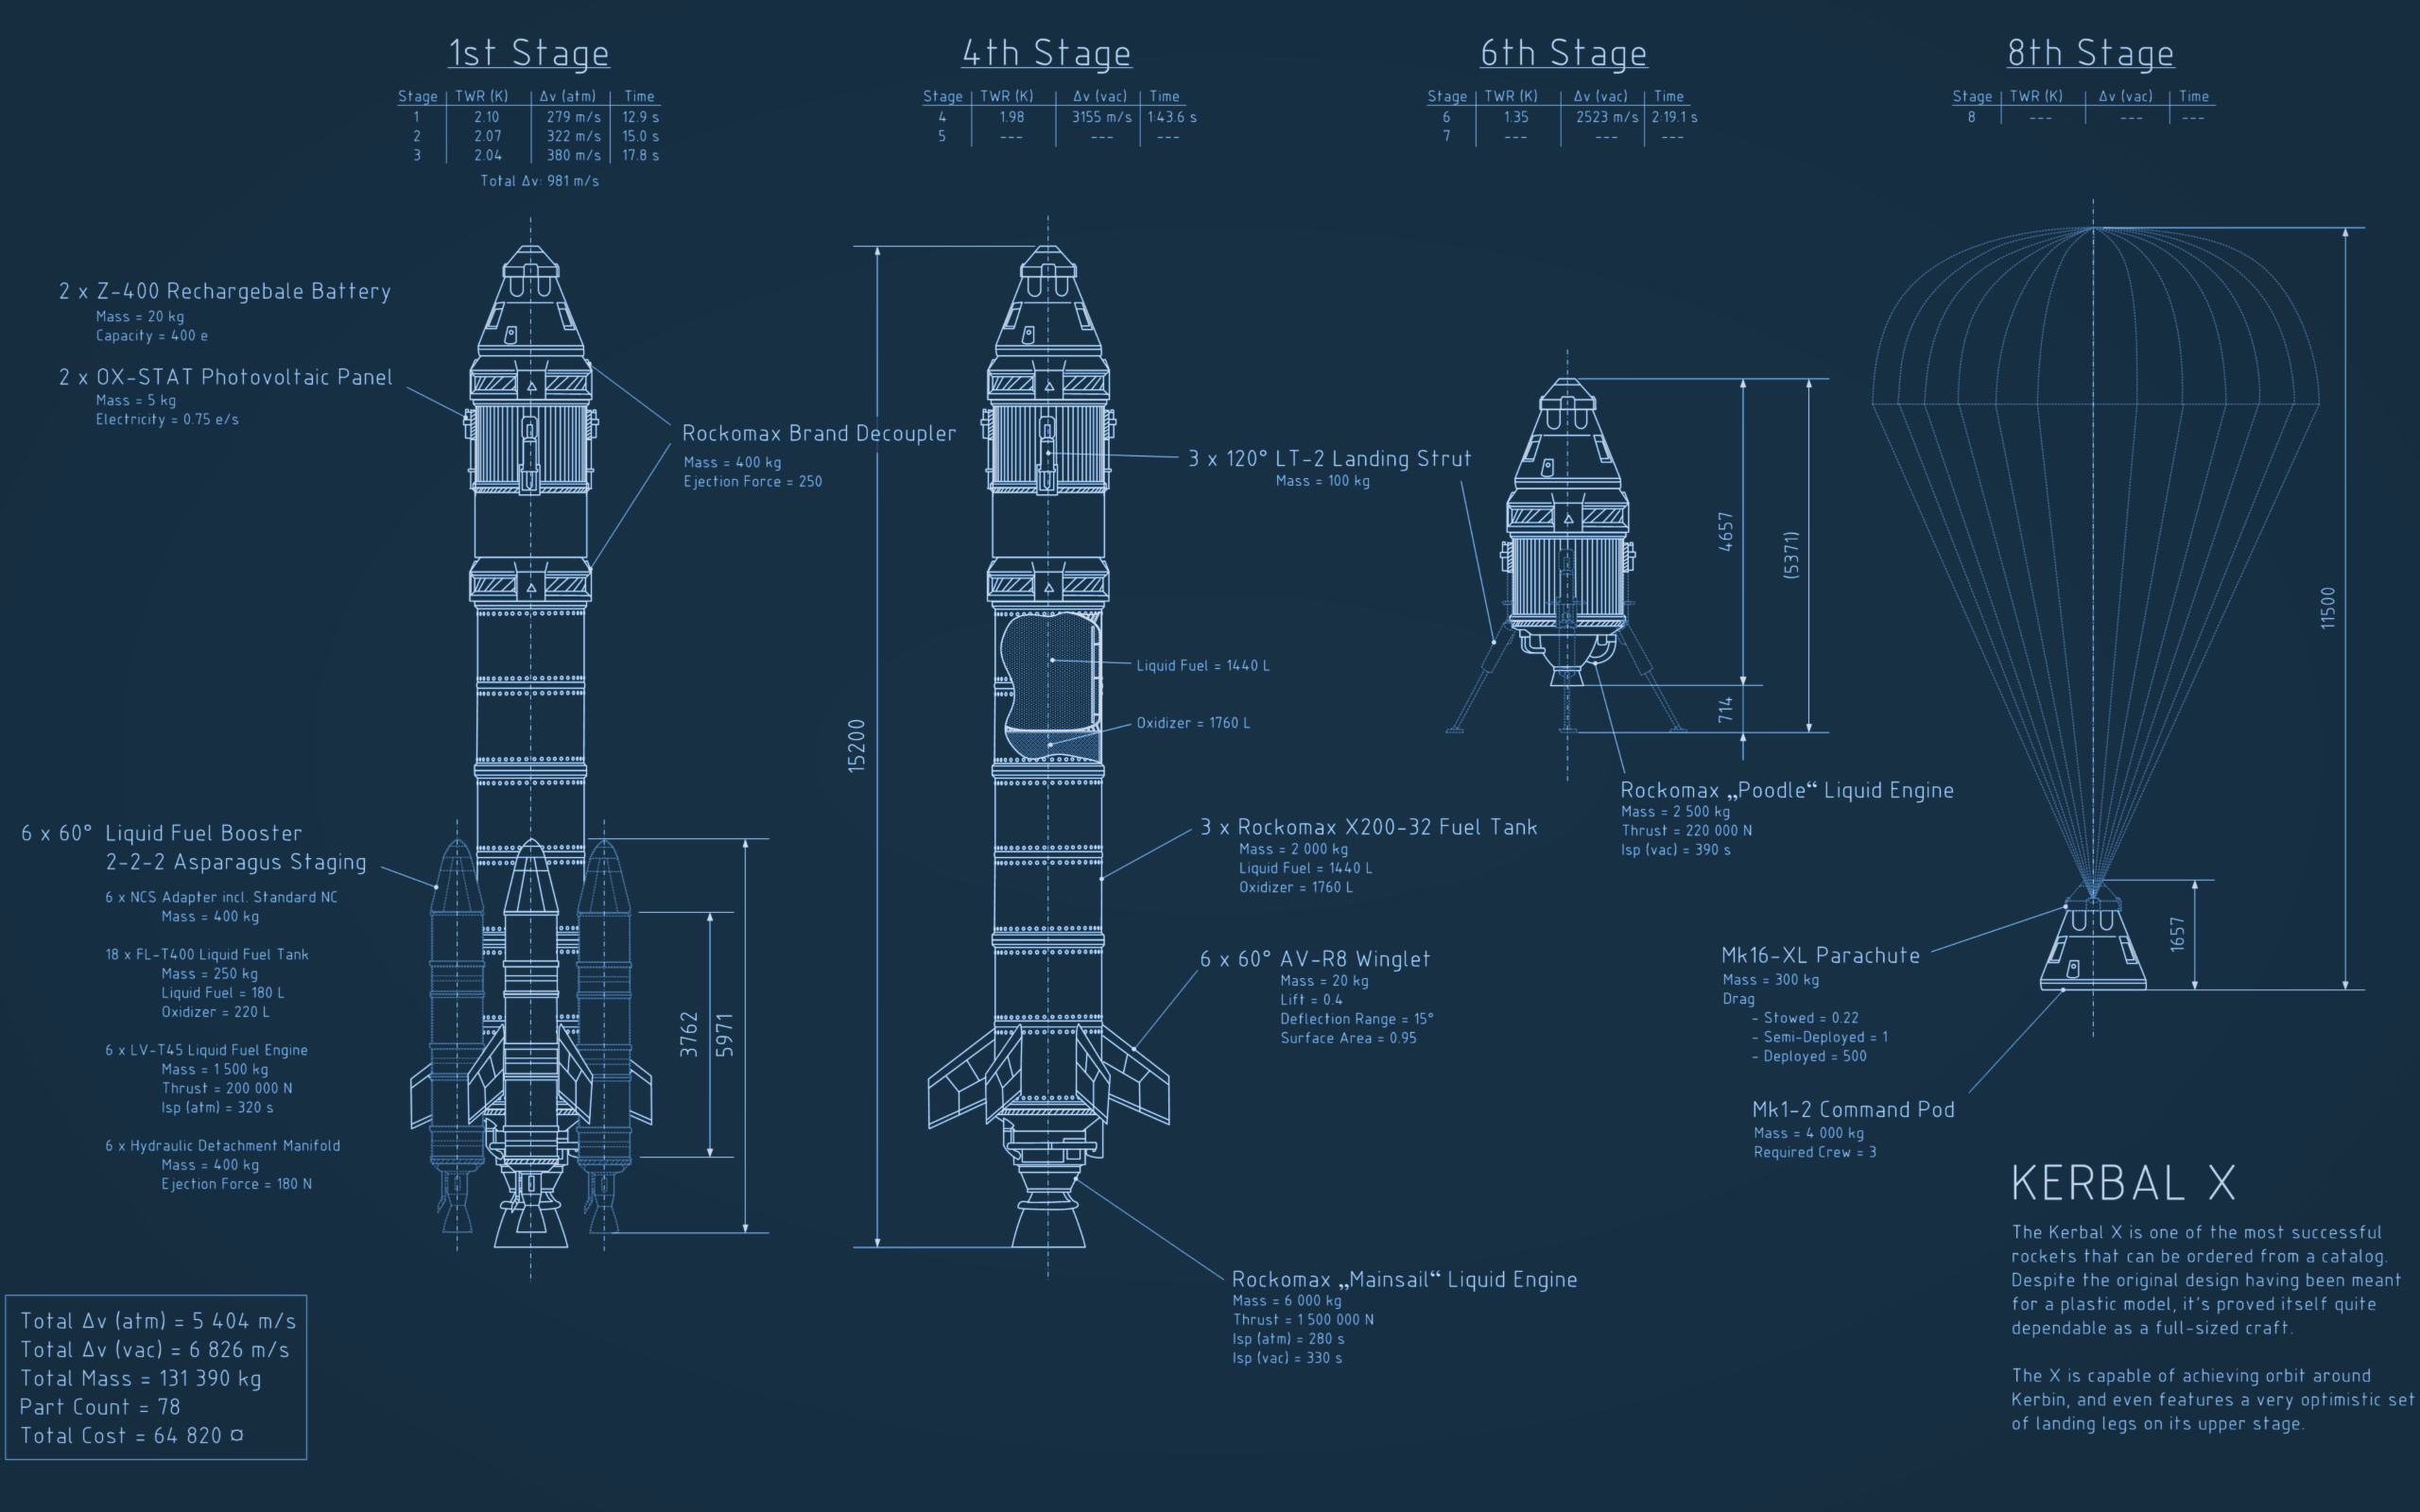
\includegraphics[width=\paperwidth]{images/staging.jpg}}%
\begin{frame}
\end{frame}
\begin{frame}
    \frametitle{Staging}
    \begin{block}{How do we do it}
        \begin{itemize}
            \item Split the rocket in 2 or more parts.
            \item Each part carries own fuel and engine
            \item Each stage can be seperated from the rocket in sequence
            \item e.g. booster stage, landing stage, transfer stage, ...
        \end{itemize}
    \end{block}
\end{frame}
\begin{frame}
    \frametitle{Staging}
    \begin{block}{Why do we do it}
        \begin{itemize}
            \item Rocket efficiency is inversly proportional to it's weight
            \item Delta-v goes up as total mass decreases (All else being equal)
            \item We want to carry as little mass as posible
            \item Throw away excess weight of unused engines and empty fueltanks
        \end{itemize}
    \end{block}
\end{frame}
}
\begin{frame}
    \frametitle{Staging}
    \begin{block}{}
        \begin{center}
            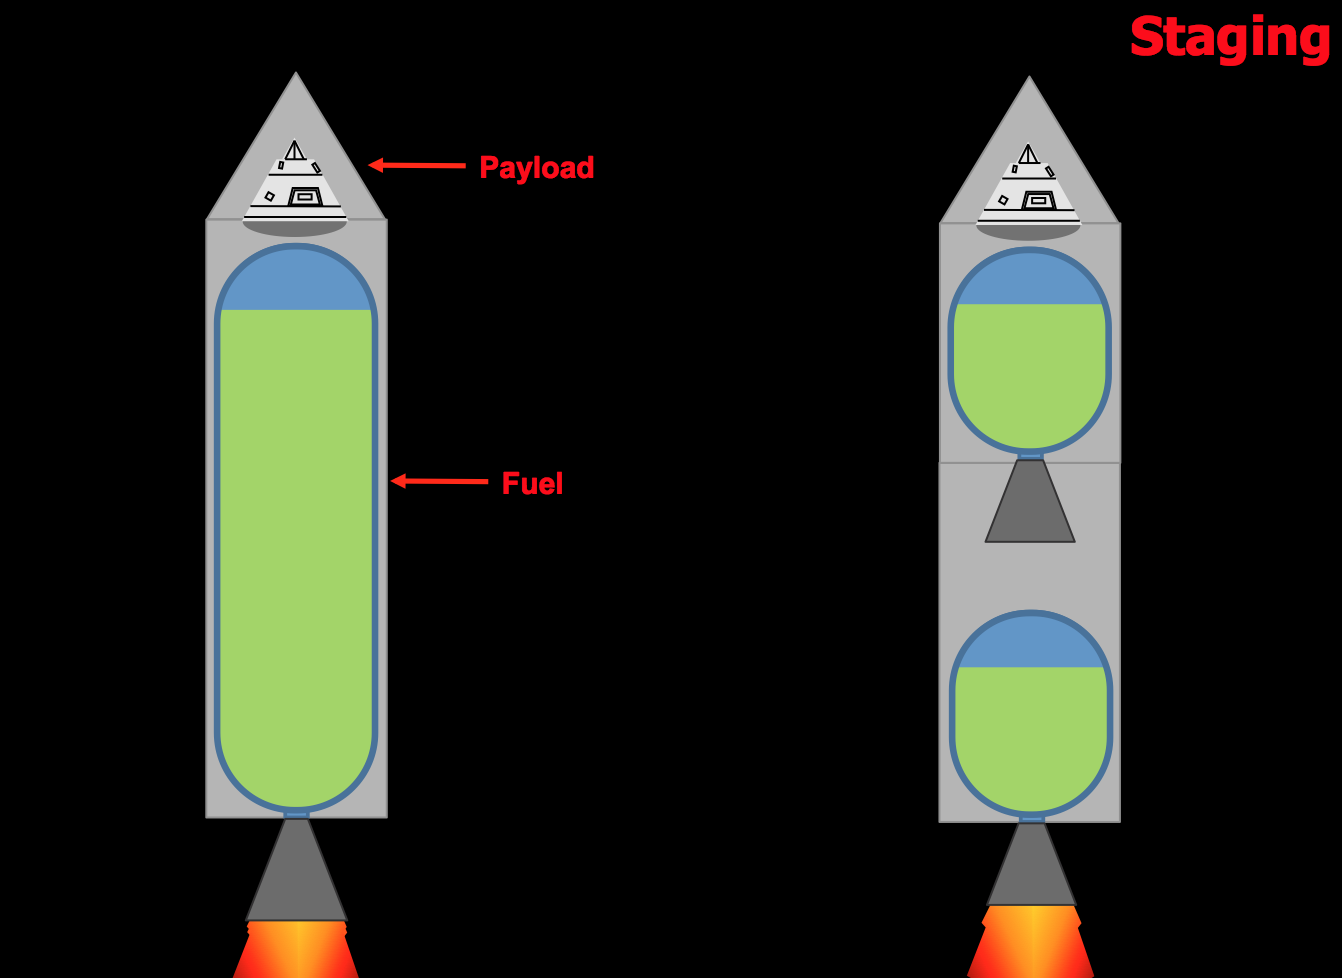
\includegraphics[width=0.5\textwidth]{images/staging1.png}
        \end{center}
    \end{block}
\end{frame}
\begin{frame}
    \frametitle{Staging}
    \begin{block}{}
        \begin{center}
            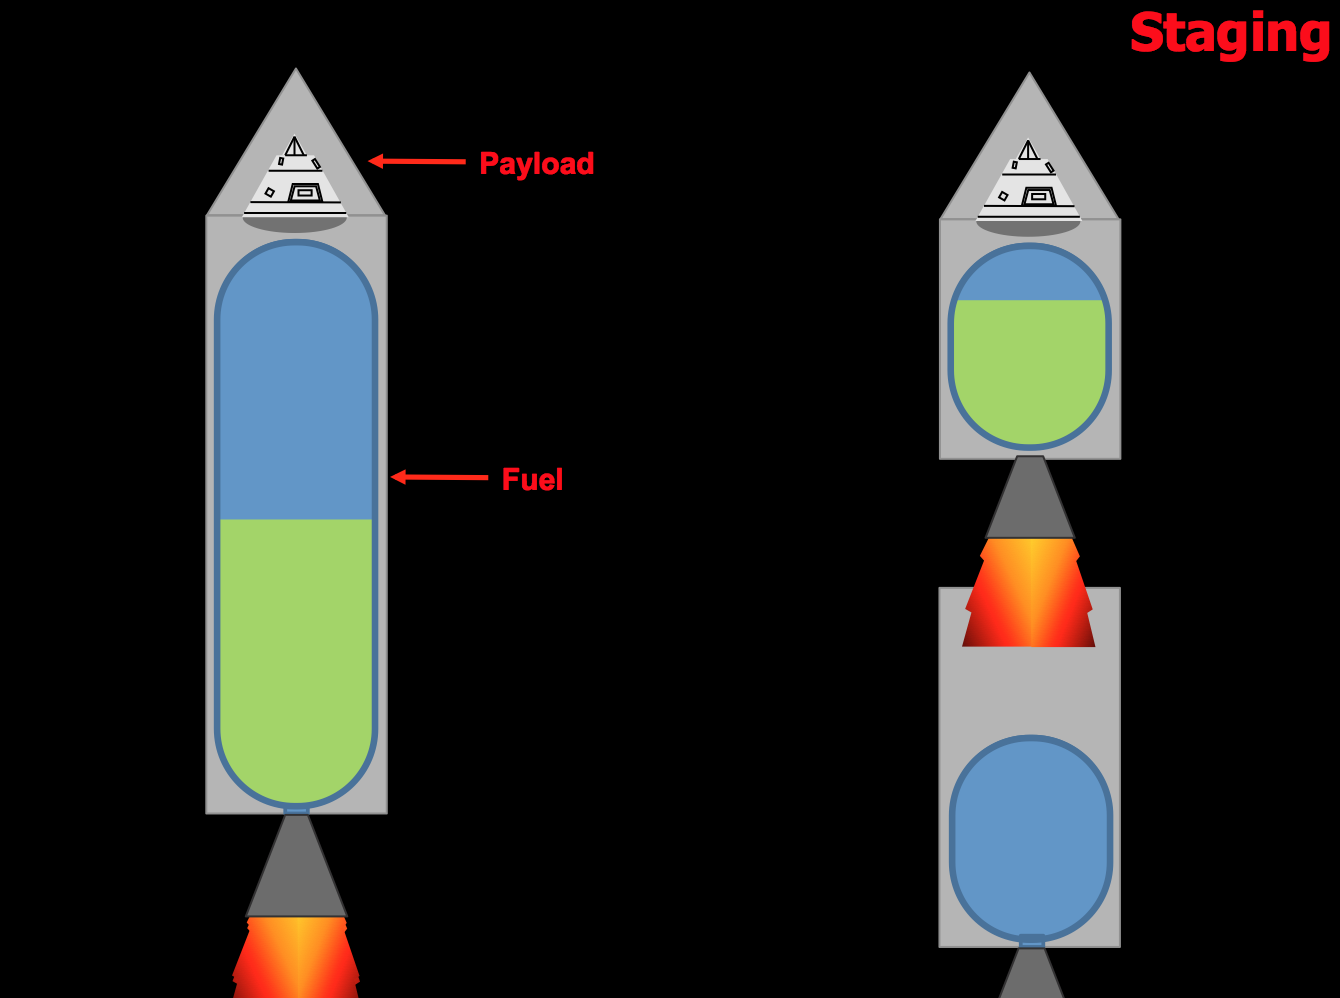
\includegraphics[width=0.5\textwidth]{images/staging2.png}
        \end{center}
    \end{block}
\end{frame}

{
\usebackgroundtemplate{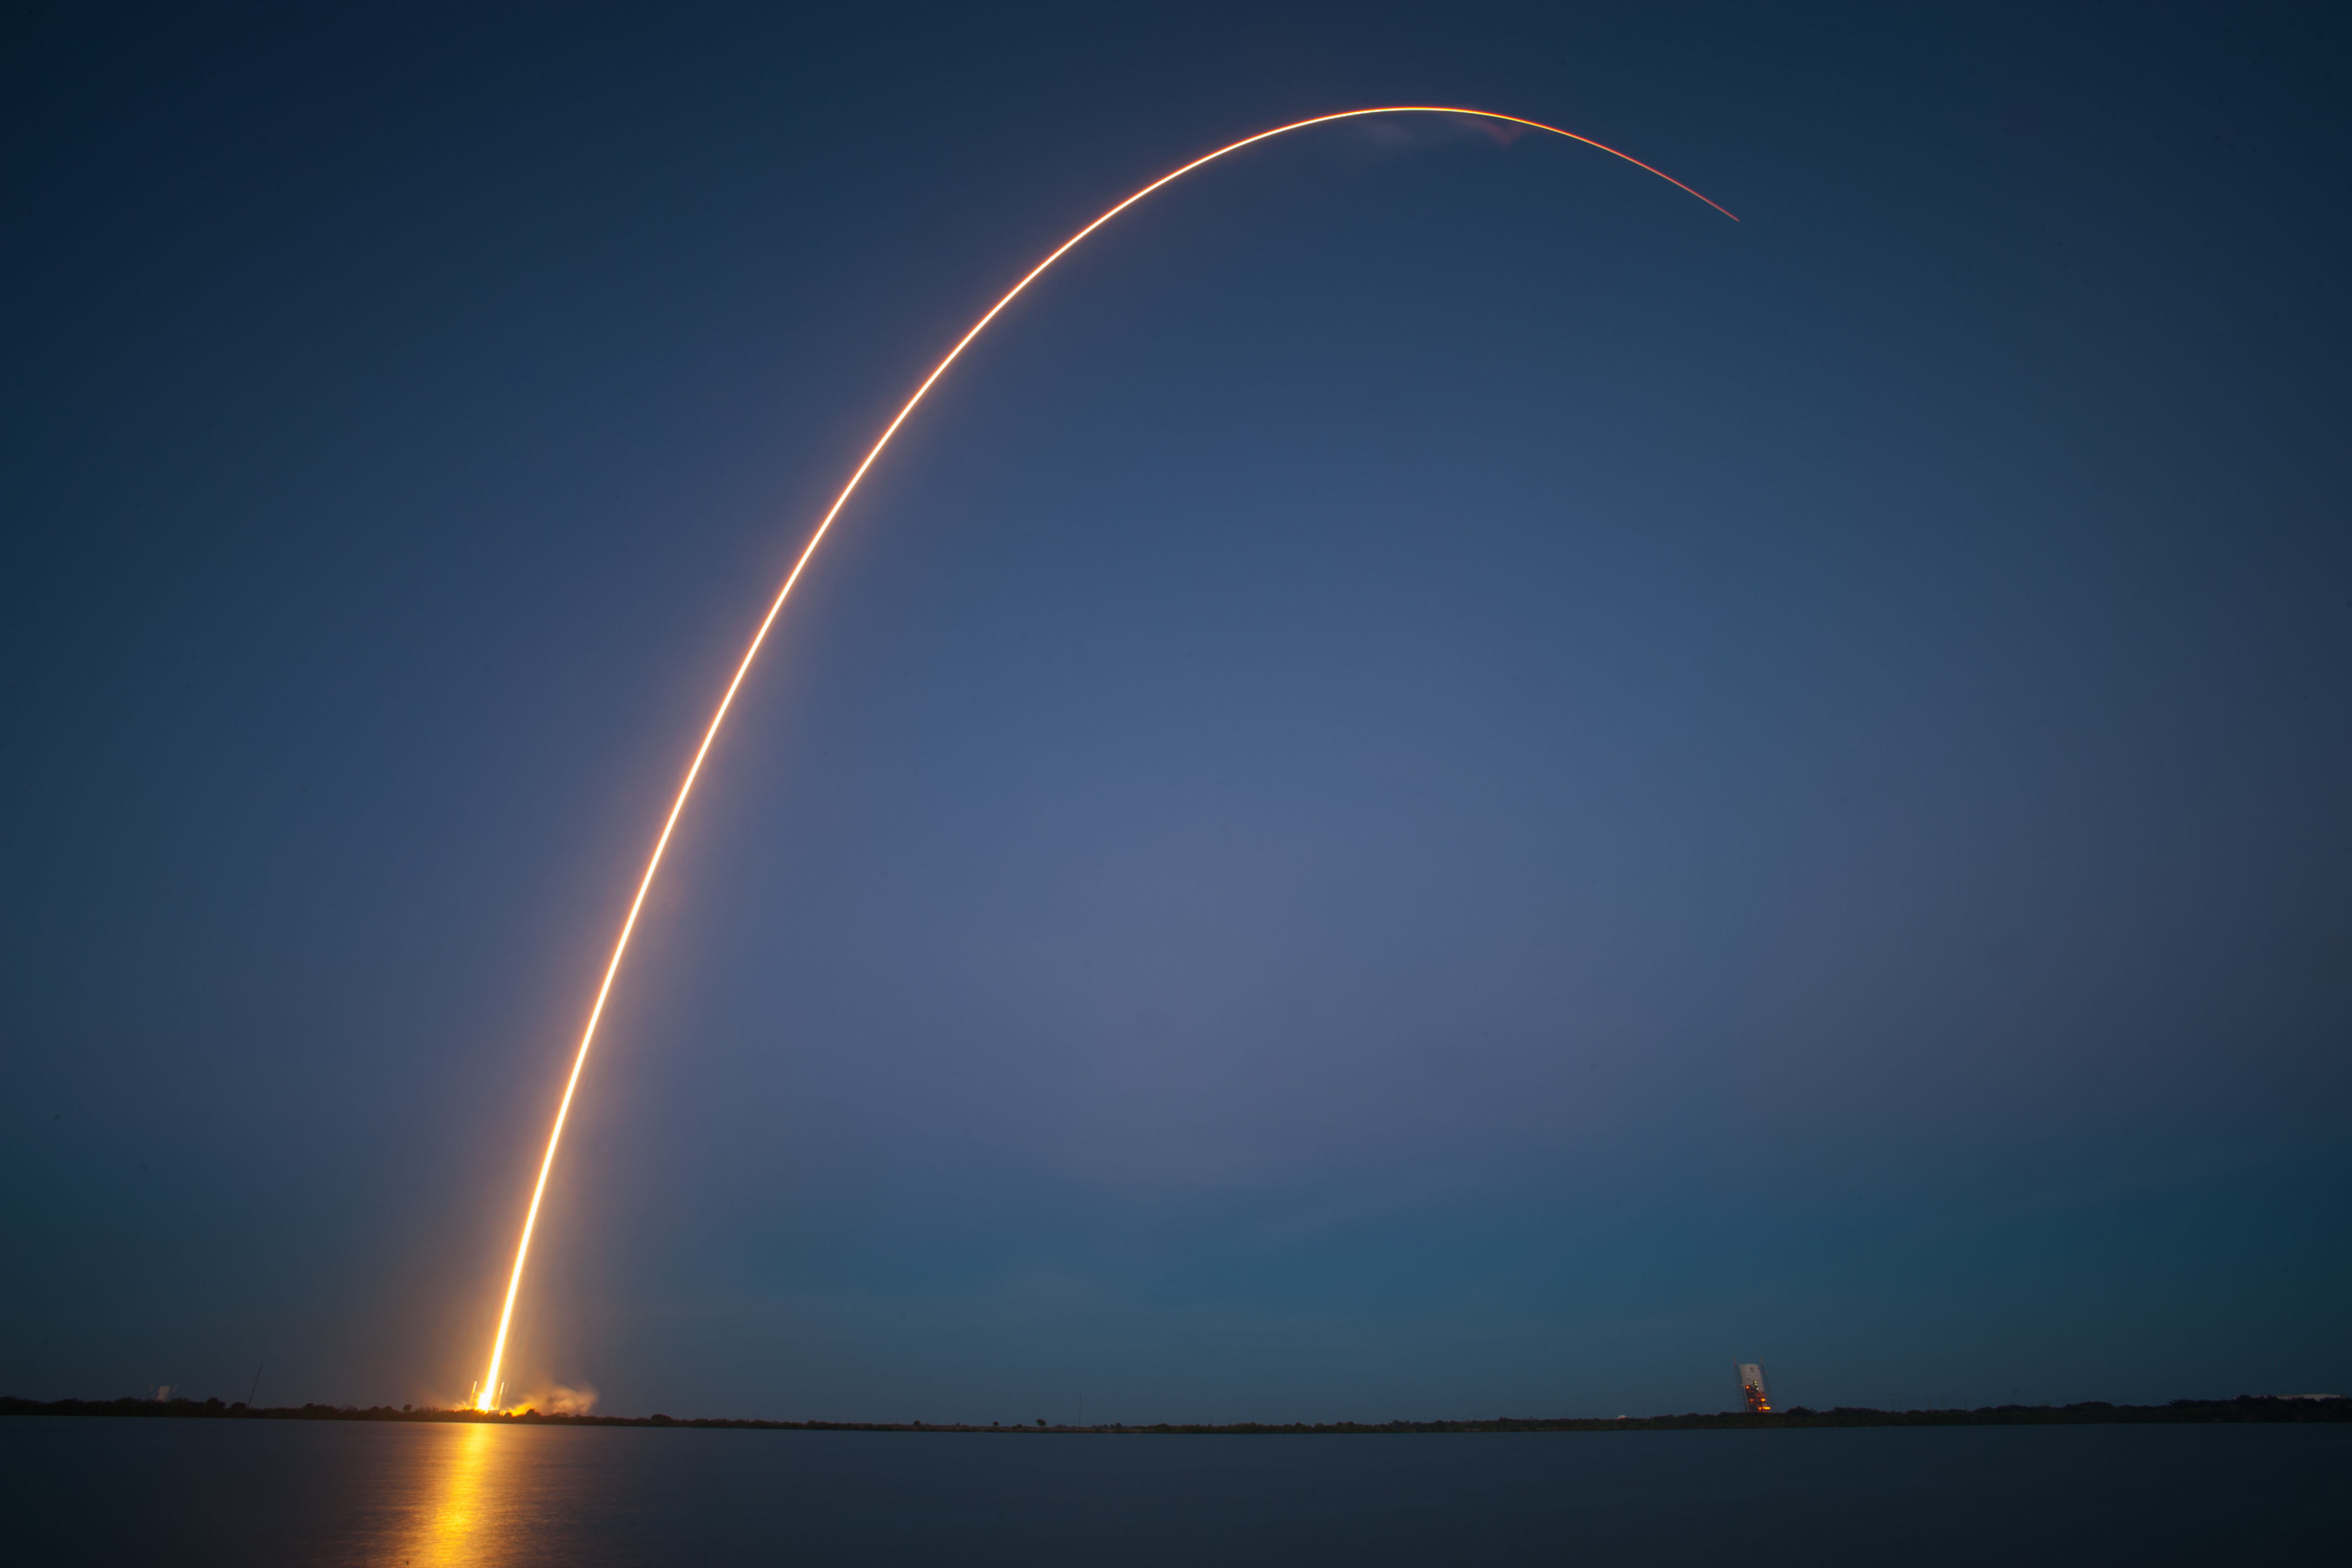
\includegraphics[width=\paperwidth]{images/gravity_turn.jpg}}%
\begin{frame}
\end{frame}
\begin{frame}
    \frametitle{Getting into orbit}
    \begin{block}{Why do we turn}
        \begin{itemize}
            \item Going straight up gains altitude quickly
            \item But we would just fall down again
            \item To get into orbit we need to move lateral as well
            \item combining vectors is efficient: $a^2+b^2=c^2$
        \end{itemize}
    \end{block}
\end{frame}
\begin{frame}
    \frametitle{}
    \begin{block}{Gravity turn}
        \begin{itemize}
            \item Rotation of earth is already moving us towards the east at 1.5km/h. Turning east saves precious delta-v
            \item rotational velocity is higher around the equator that why we want to launch from Cape Canaveral
        \end{itemize}
    \end{block}
\end{frame}
\begin{frame}
    \frametitle{Let's Launch}
    \begin{block}{How do we do it}
        \begin{itemize}
            \item throttle up
            \item point eastwards (about 5degrees)
            \item don't. touch. anything. let gravity do it's work
            \item activate staging at the appropriate times
            \item circularize orbit
            \item It easy, it's not ro... oh...
        \end{itemize}
    \end{block}
\end{frame}
}
